\section{研究方法、技术路线、实验方案}
\begin{frame}{\insertsection}
	\begin{center}
		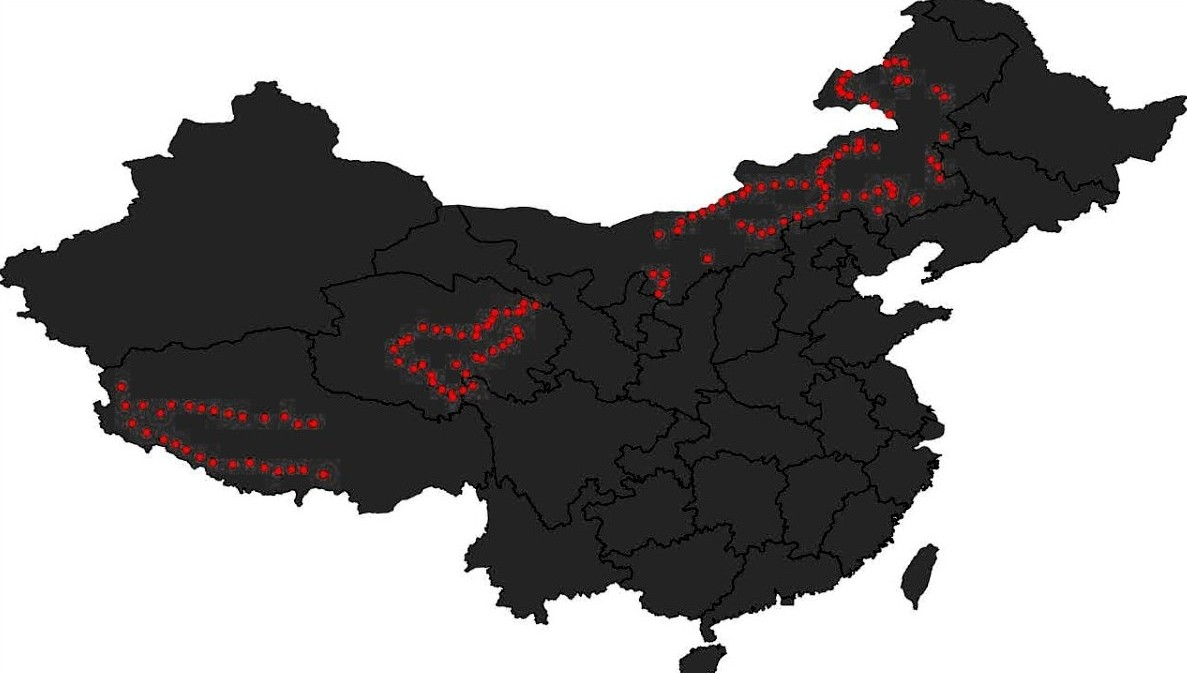
\includegraphics[width = 0.9\textwidth]{./研究方法.jpg}
	\end{center}
\end{frame}

\subsection{研究方法}
\begin{frame}{\insertsection}{\insertsubsection}
	研究地点:
	于生长季顶期分别从西藏、青海、内蒙三个省份,沿从东到西的水分梯度分成南、北两条平行样带进行采样。记录每个样点的植被类型和温度,并用GPS记录每个样点的地理坐标和海拔。
\end{frame}
\subsection{技术路线}
\begin{frame}{\insertsection}{\insertsubsection}
	\begin{center}
		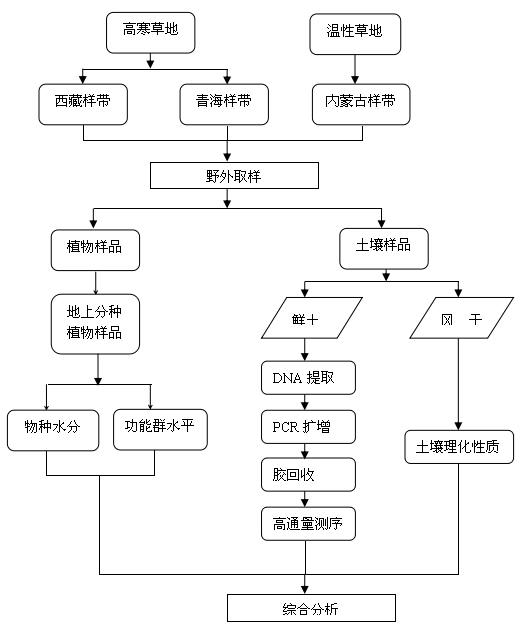
\includegraphics[width = 0.65\textwidth]{./技术路线.jpg}
	\end{center}
\end{frame}

\begin{frame}{\insertsection}{\insertsubsection}
\end{frame}
\subsection{实验方案}
\begin{frame}{\insertsection}{\insertsubsection}
\end{frame}

\begin{frame}{\insertsection}{\insertsubsection}
\end{frame}